\documentclass{thesisbeamer}

\title[Short title in footline]{The actual and probably very long title of the thesis}
\author[Name in footline]{Author \newline ~ \newline \normalsize{Advisors: Duh, Dih, Dah}}
\date{The date}

\bibliography{../biblio}

% video will work on Linux (with Okular) or OS X, for other OS's or viewers find your own way to do it
%\videoOSX	% for OS X 
\videoOFF

\begin{document}

\MakeTitleNoFoot

\begin{frame}{Introduction}
\begin{itemize}[<+->]
\item Some
\item Appearing
\item Bullets
\begin{itemize}
 \item With sub-bullets
\end{itemize}
\end{itemize} 
 \visible<+-> {
 \begin{center}
  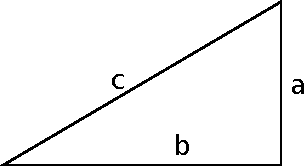
\includegraphics[width=.4\linewidth]{triangle1} \\
  And an appearing figure.
 \end{center}
 }
\end{frame}


\begin{frame}{Main content}
\begin{itemize}[<+>]
\item Some
\item Appearing
  \item And disappearing
\item Bullets
\begin{itemize}[<.>]
 \item With sub-bullets
\end{itemize}
\item That appear and disappear with their parent
\end{itemize}
\end{frame}



\begin{frame}{Main content}
\begin{enumerate}
\item Some	\vfill
\item Numbers
\begin{itemize}
 \item With sub-bullets
\end{itemize}\vfill
\item That appear and the same time\vfill
\item Nicely spaced on the slide
\end{enumerate}
\end{frame}


\begin{frame}{Citations}
 \begin{itemize}[<+->]
  \item Should be done with \textbackslash{fullcite}
  \begin{itemize}[<.->]
   \item \fullcite{pythm001}
  \end{itemize}\vfill
  \item You may also use \textbackslash{smallcite}
  \begin{itemize}[<.->]
   \item \smallcite{pythm001}
   \item It takes less space...
  \end{itemize}\vfill
  \item Check all imported references for:
  \begin{itemize}[<.->]
   \item Name / Journal name / year / editor (journals)
   \item Carefully check conference name (IEEEexplore)
  \end{itemize}
 \end{itemize}
\end{frame}

\begin{frame}{Equations}
\begin{itemize}[<+->]
  \item Have a number if used with \texttt{\textbackslash{begin}\{equation\}}
  \begin{equation}
  \forall \phi: \quad \cos ^2 \phi + \sin^2\phi = 1
  \end{equation}\vfill
  \item Do not have a number if used with \texttt{\textbackslash{begin}\{equation*\}}
    \begin{equation*}
  \forall a, b: \quad (a+b)^2 = a^2 + 2ab + b^2
  \end{equation*}
    \item Another useful environment is simply  \texttt{\textbackslash{begin}\{center\}}
    \begin{center}
    $\forall a, b: \quad (a-b)^2 = a^2 - 2ab + b^2$
    \end{center}
    \begin{itemize}[<+->]
    \item Probably more suited to slides as we use less equation references
  \end{itemize} \vfill\vfill   
  \item Can also be included in the text / bullets
  \begin{itemize}[<+->]
    \item $\forall \phi: \quad  (\cos\phi+\sin\phi)^2 = 2\cos\phi\sin\phi + 1$
  \end{itemize}
\end{itemize}
\end{frame}



\end{document}
